\documentclass[]{article}
\usepackage{lmodern}
\usepackage{amssymb,amsmath}
\usepackage{ifxetex,ifluatex}

\usepackage{scrextend} 
\usepackage[inline]{enumitem}
\usepackage{xcolor}
\usepackage{graphicx}

\usepackage{color}
\usepackage{subcaption}
\usepackage[export]{adjustbox}
\usepackage{tabularx} 



\begin{document}

\begin{center}
National Research University

Higher School of economics

Faculty of Computer Science

\vspace{25mm}
Bachelor's Programme ``HSE and University of London Double Degree
Programme in Data Science and Business Analytics''

\vspace{50mm}

\textbf{Software project report on the topic: Sentiment Analysis based on Glamping Reviews from TripAdvisors: Developing a Decision - Making Assistant''}

\vspace{35mm}

\textbf{Student:}
Morozova Milena Artemovna

\vspace{5mm}

\textbf{Supervisor:}
Chuvulina Anna Andreevna

\vspace{5mm}

\textbf{Date:}
28.05.2022

\end{center}

\clearpage


\tableofcontents
\clearpage

\section{Introduction}


\subsection{Abstract}
Over the past two years, the glamping industry in Russia has made a sharp jump. Glampings are luxury camp sites that are built in nature or even in surrounding places. But ecotourism, which is also called green tourism, involves a complete disconnection from the noise of civilization --- a rejection of the cult of comfort and mass communications. Most people, interested in glamping in Russia, are trying to find reviews on the Internet for places they would like to visit. However, reading a thousand reviews is a very long and labor-intensive process that not all people like.

Sentiment analysis allows you to determine the emotional color of a multi-line review in a matter of minutes, which greatly simplifies the choice of a glamping site for many Russian tourists.
As part of our project, we use sentimental analysis to calculate the approximate rating of the place depending on the number of reviews and their emotional coloring.

\subsection{My role in the software project}
My work was dedicated to development of a graphical user interface application, which would be as simple and understandable as possible to each user. The development of the interface includes: creating application windows and minimal application design.

Moreover, in order for the glamping rating to be reflected not only by a number, we decided to conduct a frequency analysis of reviews of each place and make a "word cloud" reflecting the most frequently used words in the texts of particular reviews. Performing frequency analysis, creating word clouds and adding them to the app was also part of my job.

As a part of collective work we decided to construct a high accuracy mathematical model, which analyses reviews and divides them into 2 categories: positive and negative. For increasing the accuracy of this model, my groupmate performed work on cleaning, tokenization, lemmatization of text, as well as filtering and removing words that do not give emotional color to the text.

\subsection{Instruments}

\begin{enumerate} 
	\item Anaconda, Jupiter Notebook, Pycharm
	\item Python libraries: numpy, pandas, matplotlib, sklearn, scipy,wordCloud
	\item Microsoft Excel
	\item PyQt, Qt Designer
	\item TextBlob
	\item TripAdvisor
	
\end{enumerate}

\subsection{Main goal}
The main goal of our application is to perform the sentiment analysis and to calculate rating of glamping places in Russia in order to help tourists with their choice.

\section{Review and comparative analysis}
\subsection{Review of abstracts which you used for project and review of analogues}

The project is dedicated to learning how to filter the text and use it in different purposes, also we have learned how to increase the accuracy of mathematical models. To create the app we need to use our knowledge of GUI development and some kind of design. We have not found any exact analogues to the application we created. Of course, there are many applications that compare, for example, hotels or air tickets at a price, but the purpose of our application is to assess a specific place and acquaint the user with the words and phrases that visitors of glamping most often used to describe a particular resort. Thanks to this approach, the user will be able to quickly and accurately determine what place he will like without rereading hundreds of reviews on the Internet. And also, since glamping is a relatively new direction for Russia in the field of tourism, there are few reviews for glamping, they are scattered throughout the Internet, and our application allows you to structure all reviews so that the user can find out all the information he needs in one place just by clicking on the button.
Now I will compare our application with an application called ``Twitter Sentiment analyzer''. It is a distant analogue of our application and analyzes the emotional coloring of statements on Twitter. 

\vspace{5mm}

\begin{tabularx}{335pt}{|c|X|c|X|c|}

\hline
\textbf{Characteristics} & \textbf{Twitter Sentiment Analyzer} & \textbf{a Decision-Making Assistant}\\\hline

Paid/Free & Paid & Free\\\hline

Visualization & Short video clips & Calculated rating and word clouds\\\hline

Used for & Analyzing the product reviews & Analyzing glamping places\\\hline
\end{tabularx}

\subsection{List of key words}

\texttt{Sentiment Analysis}
--- determining the polarity of emotional assessments in the text under study, which contains opinions, judgments, emotions, the author's attitude to entities, personalities, questions, events, topics and their attributes.\vspace{3mm}

\texttt{A machine learning model}
--- a file that is trained to recognize certain types of patterns. You train a model based on a dataset, providing it with an algorithm that it can use to analyze and learn from that data.\vspace{3mm}

\texttt{Graphical User Interface(GUI)}
--- a system of tools for user interaction with electronic devices, based on the presentation of all system objects and functions available to the user in the form of graphic components of the screen (windows, icons, menus, buttons, lists, etc.).\vspace{3mm}

\texttt{A recurrent neural network(RNN)}
--- is a class of artificial neural networks in which connections between nodes form a directed or undirected graph along a time sequence. This allows her to exhibit temporary dynamic behavior. Derived from direct communication neural networks, RNNs can use their internal state (memory) to process sequences of variable-length input data.\vspace{3mm}

\texttt{Dataset for machine learning}
--- processed and structured information in tabular form.\vspace{3mm}

\texttt{Long short-term memory (LSTM)}
--- a special type of recurrent neural network architecture capable of learning long-term dependencies.


\section{Selection of methods, algorithms, and models for project implementation}

\subsection{Information about the given data}
Firstly, I got unfiltered data called ‘data.csv’ in the format of .csv which I opened in Microsoft Excel. The dataset contains data from “TripAdvisor” --- the website, containing the reviews about hotels, restaurants, glamping etc. 
In the original unfiltered csv file, we have two columns: the name of the place and the feedback about it. Working with the unfiltered data set, we receive information that we need later for work, namely: the number of places for glamping and their names and the number of reviews for each specific place.

\subsection{Purifying data for analysis and processing}
Any text data in its raw material form cannot be analyzed by NLP libraries. This data must be cleaned using various data processing techniques. This part of work was done by my groupmate, so I will describe it quite briefly in my report and focus on describing my work.In this project, we used standard processing methods used for sentimental analysis, namely:

\begin{itemize}
\item
  \texttt{Eliminate HTML Tags:}
  Unstructured Text Contains a lot of "noise" and therefore we need to remove HTML tags, if any.
\item
  \texttt{Eliminate special characters:}
  Any non-alphanumeric characters in the text must be removed.
\item
  \texttt{Deleting stop words:}
  Stop words are commonly used words (i.e., "the," "a," "an") that do not add meaning to a sentence and can be ignored without significantly affecting the meaning of the sentence.
\item
  \texttt{Lemmatization:}
  We implemented lemmatization with Spacy so that we could count the appearance of each word. Lemmatization removes grammatical time and transforms each word into its original form. Another way to convert words to its original form is called stemming. Although stemming takes the language root of the word, lemmatization takes the word into its original lemma. For example, if we did contrary to the word "apples," then we would get "appl," while lemmatization would give us "apple." Therefore, we used lemmatization instead of stemming, as it is much easier to interpret.
  
\end{itemize}

\subsection{Preparing training data for the future model}
To prepare the data and to build the model we are using Keras.
Keras is a deep learning library, which is a high-level API written in Python and capable of running on top of TensorFlow, Theano or CNTK. It was designed with the expectation of rapid learning.
To train the model, we will use two sets of data that we will later combine - one contains only positive statements, the second --- negative ones.

Let's start by importing the necessary dependencies to preprocess the data and build the model:
\vspace{2mm}

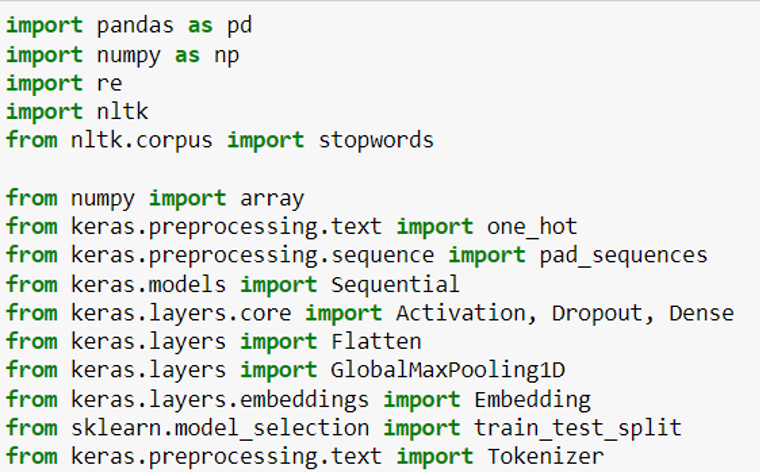
\includegraphics[width=0.5\textwidth, center]{images/pict1.png}

\vspace{4mm}
Now let's download texts with positive and negative statements (they will be in separate files: train\underline{\hspace{1mm}}data\underline{\hspace{1mm}}true and train\underline{\hspace{1mm}}data\underline{\hspace{1mm}}false). Next, we will immediately combine the lists of statements into a single list and calculate the length of each of them(Look at \label{fig:figure1} ).Then we need to break these statements into words. To do this, we will use the \texttt{Tokenizer} tool and assume that the maximum number of words will be 2000.

This parameter has one significant plus: of all the words found, we leave 1999 most frequently encountered, that is, we discard rare words that are not particularly needed when learning the neural network. 

For example, with a large training sample, a good choice would be a value within 15000-20000.
While splitting the text into words, we remove all punctuation signs and unnecessary characters, and also bring all our words to the lower case.

\clearpage

\begin{figure}
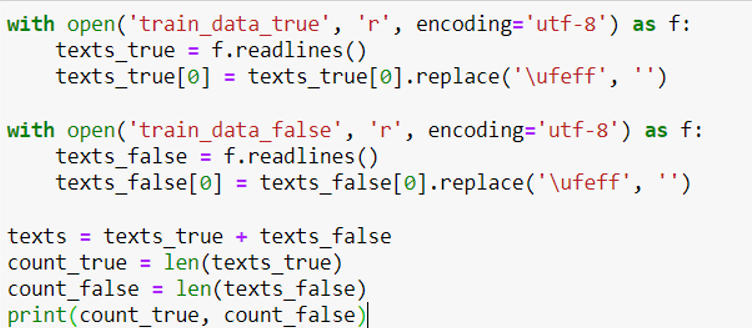
\includegraphics[width=\textwidth]{images/pict2.png}
\caption{Downloading texts}
\vspace{3mm}
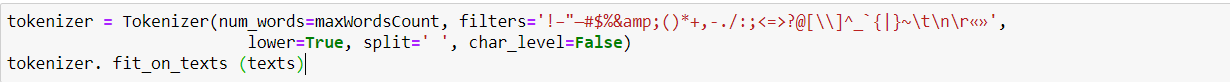
\includegraphics[width=\textwidth]{images/pict3.png}
\caption{Breaking into words}
\label{fig:figure1}
\end{figure}


Next, we convert the text into a sequence of numbers in accordance with the resulting dictionary. To do this, I used a special method of the Tokenizer class:
\vspace{2mm}

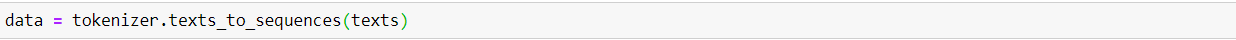
\includegraphics[width=\textwidth]{images/pict4.png}
\vspace{3mm}

At the output, we get a two-dimensional array of numbers of the numpy object. Now, we need to align all these vectors to a length equal to the maximum length of the text. To do this, another built-in pad\underline{\hspace{1mm}}sequences method is used, which trims the data array to a length of max\underline{\hspace{1mm}}text\underline{\hspace{1mm}}len and adds zeros for short vectors.(Look at \ref{fig:figure2})
\vspace{2mm}

As we can see, for too short phrases zeros were added at the beginning of the vectors. We obtained a two-dimensional training sample tensor. Let's form another tensor for the required output values  of the network. We will encode the answers according to the following rule(Picture \ref{fig:figure3})

\clearpage

\begin{figure}
\begin{subfigure}{0.4\textwidth}
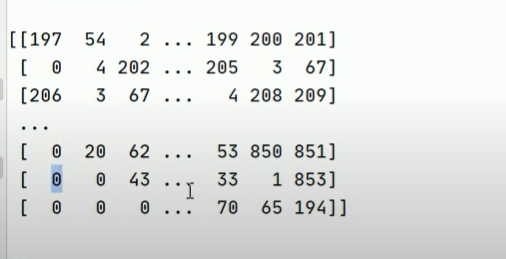
\includegraphics[width=0.9\linewidth, height=4cm]{images/pict5.png}
\caption{Vectorized text}
\label{fig:figure2}
\end{subfigure}
\begin{subfigure}{0.6\textwidth}
\includegraphics[width=0.9\linewidth, height=4cm]{images/pict6.jpg}
\caption{Encoding rule}
\label{fig:figure3}
\end{subfigure}
\caption{Text coding and vectorization}
\end{figure}

Our neural network will have 2 neurons at the output - the upper neuron will be responsible for the positive text, the lower - for the negative. For positive statements at the output, we will require the vector [1.0], respectively for negative - [0.1]. For example, we know that in our collection data\underline{\hspace{1mm}}pad first all positive statements go, and then all negative ones, and we can also find out their number using the count function. Using this number, we will form the output vector we need.

We generate a set of such outputs as follows:

\vspace{2mm}
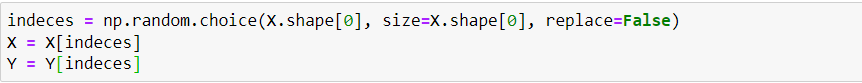
\includegraphics[width=0.7\textwidth, left]{images/pict7.png}

\vspace{2mm}
Now we have a training sample and the required output values. For better training, we mix all these statements so that mixed and positive and negative are submitted to the entrance. So the network will be better trained:

\vspace{2mm}
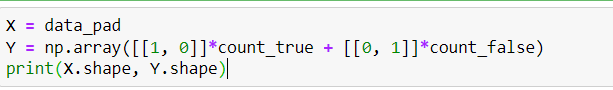
\includegraphics[width=0.7\textwidth, left]{images/pict8.png}

\vspace{3mm}
\subsection{Creating a Reccurence Network Model}

To create a recurrent network model, we will use the LSTM recurrent layer. To create it in Keras, we use the class:

\vspace{2mm}
\textbf{keras.layers.LSTM(units,\dots)}

\vspace{2mm}
As the first parameter (units), the number of neurons in each fully connected layer inside the LSTM cell is indicated:

\vspace{2mm}
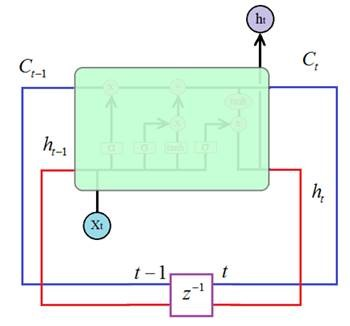
\includegraphics[width=0.8\textwidth, center]{images/pict9.jpg}

\vspace{2mm}
They will also form the dimension of the output vector. For example, let's create an LSTM layer with 64 neurons. Then the dimension of the output vector will be 64 elements. Next, let's add another same layer with 32 neurons. We will get a stack of two recurrent layers.

At the output, we will put a fully connected layer with two neurons and the softmax activation function. Let's define Adam optimization with a convergence step of 0.0001.

After we have started the learning process,to check whether our model works, we will form some text and convert it to the input format of our network.

Firstly, we add an auxiliary function. When preparing the text, we formed a dictionary in which indexes first go, and then words. With this dictionary, our function sequence\underline{\hspace{1mm}}to\underline{\hspace{1mm}}text converts a sequence of indexes back into words:

\vspace{2mm}
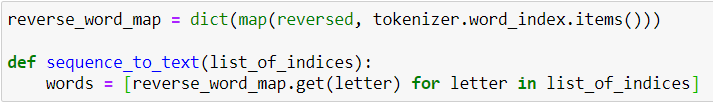
\includegraphics[width=0.8\textwidth, center]{images/pict10.png}

\vspace{2mm}
Then we test the model(Picture \ref{fig:figure4}) and finally obtain the result(Picture \ref{fig:figure5})

\vspace{2mm}
\begin{figure}
\begin{subfigure}{0.5\textwidth}
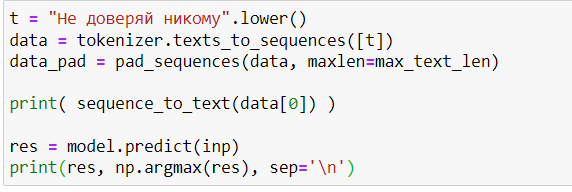
\includegraphics[width= 1\linewidth, height=3cm]{images/pict11.png}
\caption{Testing the model}
\label{fig:figure4}
\end{subfigure}
\begin{subfigure}{0.5\textwidth}
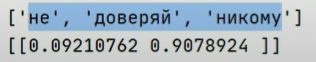
\includegraphics[width=1\linewidth, height=3cm]{images/pict12.png}
\caption{Result}
\label{fig:figure5}
\end{subfigure}
\caption{Final stage}
\end{figure}

\vspace{2mm}
It can be noted that we have the greatest value in the resulting vector on the second neuron, and the vector itself is close to the vector [0.1], which we demanded precisely for negative statements, therefore the expression has a negative emotional color.

\vspace{3mm}
\subsection{Word Clouds}
As we have already purified out data, then it is quite easy to create a word cloud for every particular place.

To do this, we use the WordСloud package. The WordСloud package in Python helps us find out the frequency of a word in text content using rendering. We use this visualization because the cloud shows the most popular words of the text, which is useful for quickly evaluating it.
I have tested the WordCloud on a random filtered dataset and obtained the following result:

\vspace{2mm}
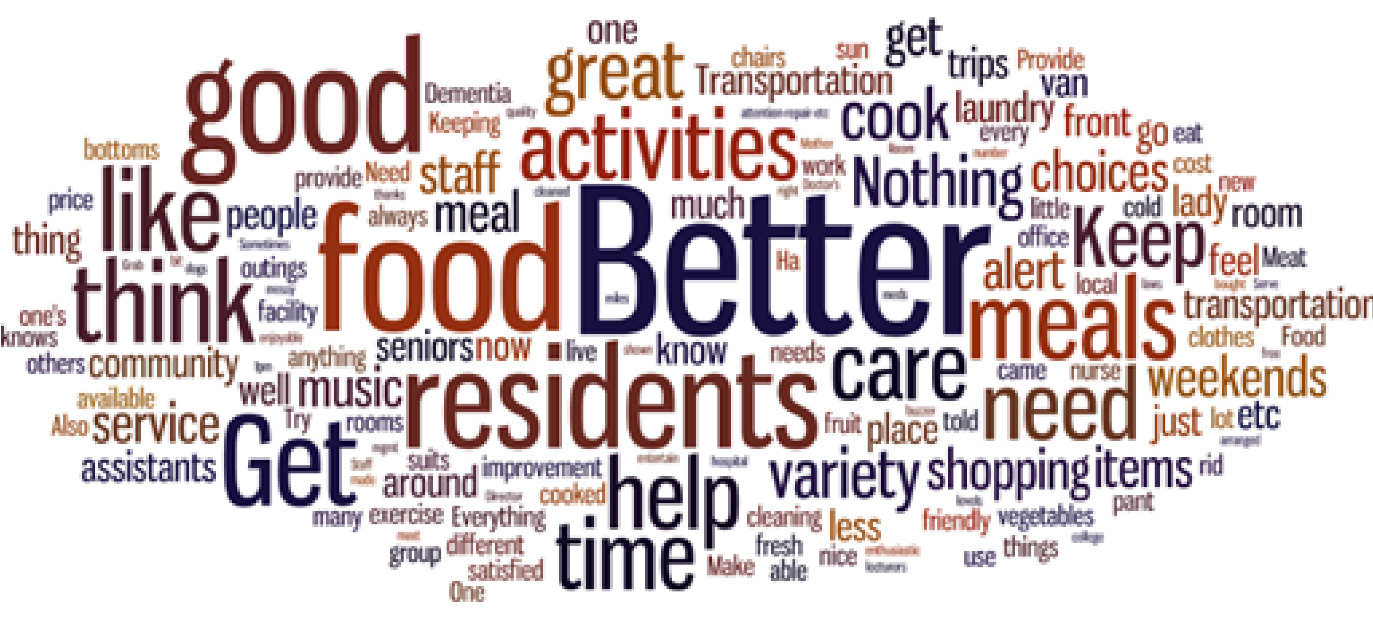
\includegraphics[width=0.8\textwidth, center]{images/pict14.png}

\subsection{GUI Application}
The next step is creating the graphical user interface with the help of PyQt and QtDesigner.
Instead of using fixed positions and element sizes in the application, we use layouts, since fixed positions and dimensions will only look good until the window is resized, and with fixed positions we cannot be sure that everything will be the same on other machines and/or operating systems. Layouts are containers for widgets that will keep them in a certain position relative to other elements. Therefore, when changing the size of the window, the size of widgets will also change.

\vspace{2mm}
In our application we have:

\begin{enumerate}
	\item The Icon
	\item The main window, where we have the name of the application, the string in which the dataset should be entered and the clickable button to start the application.
	\item After the user clicks the button, a new window appears on the screen, which on each new line contains the name of the glamping place available in the dataset. The name of each place has a button near it so that the user can choose a specific place, information about which he wants to find out.
	\item 	When the user clicks on one of the names, a new window opens containing information about this place, namely: 
	
	\begin{enumerate}
		\item The total number of reviews.
		\item The number of positive reviews.
		\item Rating of this place calculated by the program.
		\item Cloud of words showing the most common words in reviews.
	\end{enumerate}
\end{enumerate}

All additional code can be found here:

\url{https://github.com/MorozovaMilena/Project-2-course}

\vspace{3mm}
\subsection{Formulas}
I do not have any formulas in my project, so these are arbitrary formulas from chemistry, physics etc.

\[E_p=E_0-\frac{RT}{nF}\ln\left(\frac{C(K_4[Fe(CN)_6])}{K_4[Fe(CN)_6]}\right)\]

\vspace{2mm}

\Large $FWHM = \sqrt{(\frac{0.88\lambda_{em}}{n-\sqrt{(n^2-NA^2)}})^2+(\frac{nPH\sqrt{2}}{NA^2})^2}$ 

\vspace{2mm}

\[p_{\theta}(x) = \frac{\theta^{\beta} x^{\beta-1}}{\Gamma(\beta)} e^{-\theta x}\]

\vspace{2mm}


\section{Results and Conclusion}
In the software project I have significantly improved my GUI development skills, got acquainted with many useful libraries, such as, for example, WordCloud, TextBlob, Keras and Scipy. Moreover, by observing and participating a little in the part of the work that was devoted to cleaning text, I have learned many new methods and algorithms that make it much easier to work with data. Global work has been done with mathematical models. Models and classifiers based on theorems that we studied in different subjects of the 2nd course (Mathematical statistics, Discrete mathematics, and so on) were studied. In the process of studying mathematical models, were identified several factors that affect their accuracy, which was very useful to learn in order to be able to independently improve the accuracy of these models.
\clearpage

\section{Bibliography}

\begin{itemize}
\item Machine Learning, Neural and Statistical Classification 

\url{https://www1.maths.leeds.ac.uk/~charles/statlog/}

\item Cleaning & Preprocessing Text Data for Sentiment Analysis 

\url{https://towardsdatascience.com/cleaning-preprocessing-text-data-for-sentiment-analysis-382a41f150d6}

\item Generating WordClouds in Python Tutorial 

\url{https://www.datacamp.com/tutorial/wordcloud-python}

\item TripAdvisor

\url{https://www.tripadvisor.ru/}

\item Sentiment Analysis of Review Datasets Using Naïve Bayes‘ and K-NN Classifier 

\url{https://www.researchgate.net/publication}

\item Implementing Naive Bayes for Sentiment Analysis in Python 

\url{https://medium.datadriveninvestor.com/implementing-naive-bayes-for-sentiment-analysis-in-python-951fa8dcd928}

\item Keras Documentation

\url{https://ru-keras.com/recurrent-layers/}

\item Python GUI(PyQt and Qt Designer)

\url{https://tproger.ru/translations/python-gui-pyqt/}
\end{itemize}


 
\end{document}
